\section{Temporal-Difference Learning}

TD learning is novel to RL. It is a hybrid that lies between monte carlo and dynamic programming methods. As with those, TD learning uses GPI; control (policy improvement) works in much the same way, it is in the prediction of the value function (policy evaluation) where the distinctions lie.

\subsection{TD Prediction}
Monte carlo methods wait until the end of the episode before back-propagating the return to the states visited en-route. The simplest TD method (TD(0)) does not wait until the end of the episode, in fact, it updates its estimate of the value function $V(s)$ based on the instantaneous reward as follows:
\begin{equation} \label{eq: td}
V(S_t) \leftarrow V(S_t) + \alpha \left[R_{t+1} + \gamma V(S_{t+1}) - V(S_t)\right]
\end{equation}

Note here, that TD(0) \textit{bootstraps} in much the same way DP methods do i.e. it bases it's estimate of $V(s)$ on the value of the next state $V(s')$. TD methods therefore take both sampling from monte carlo, and bootstrapping from DP. The TD(0) backup diagram is shown in Figure \ref{fig:td(0)}.

\begin{figure}[h!]
	\centering
	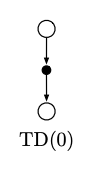
\includegraphics[width=0.2\textwidth]{/chapter6_1}
	\caption{Backup diagram for TD(0)}
	\label{fig:td(0)}
\end{figure}

The quantity in the brackets of equation \ref{eq: td} is known as the \textit{TD error}. Formally this is expressed as:
\begin{equation}
\delta_t = R_{t+1} + \gamma V(S_{t+1}) - V(S_t)
\end{equation}

\begin{figure}[h!]
	\centering
	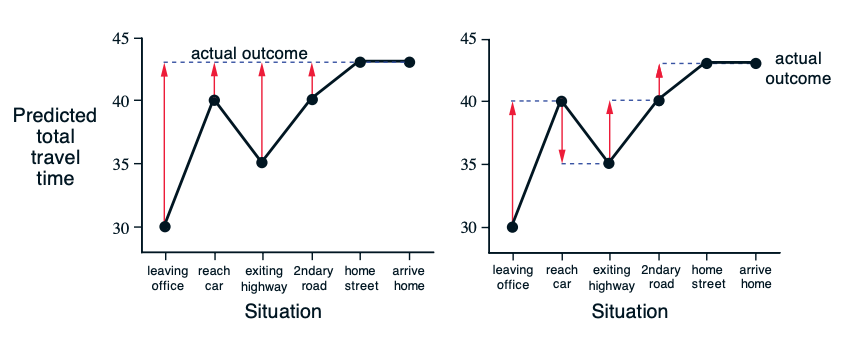
\includegraphics[width=\textwidth]{/chapter6_2}
	\caption{Monte carlo updates (left) and TD-updates (right) to the value function associated with a daily commute}
	\label{fig:td vs. mc}
\end{figure}

In Figure \ref{fig:td vs. mc} we see the differences between monte carlo and TD updates to the value function. In the case of monte carlo, we would need to wait until we arrived home before we could update our predictions for journey length. With TD learning, we can adjust these estimates on the fly based on the error in our predictions en-route. We see here that the adjustment we make changes at each timestep depending on the difference between predictions, that is to say, the update is proportional to the \textit{temporal differences} between our predictions across timesteps.

\subsection{Advantages of TD Prediction Methods}
\begin{itemize}
\item TD methods generally converge faster than MC methods, although this has not been formally proven.
\item TD methods do converge on the value function with a sufficiently small step size parameter, or with a decreasing stepsize.
\item They are extremely useful for continuing tasks that cannot be broken down in episodes as required by MC methods.
\end{itemize}

\subsection{Optimality of TD(0)}
If we only have a finite number of episodes or training data to learn from we can update our value function in \textit{batches}. We repeatedly play the same data, and update our value function by the sum of each of the increments for each state at the end of the batch.

TD batching and Monte Carlo batching converge often on two different estimates of the value function. The monte carlo batch estimate can only judge based on observed rewards from a state, but TD batching can make estimates based on later states using bootstrapping. Example 6.4 (\textit{You are the predictor}) on pg 127 explains this excellently. The monte carlo estimate will converge on the correct estimate of the value function produced by the training data, but TD methods will generalise better to future rewards because they preserve the transition from state-to-state in the TD update, and thus bootstrap better from values of other states.

In general batch MC methods always minimise the mean squared error or the training set whereas TD(0) finds the estimates that would be exactly correct for the maximum-likelihood model of the Markov process. This is called the \textit{certainty equivalence estimate} because it is equivalent to assuming that the estimate of the underlying process was known with certainty rather than being approximated.

\subsection{Sarsa: On-policy TD Control}
We'll now look at using TD prediction methods for control. We'll follow, as before, the framework of Generalised Policy Iteration (GPI), only this time using TD methods for predicting the value function.
For on-policy control, we wish to learn the state-action value function for our policy $q_\pi(s,a)$ and all states $s$ and actions $a$. We amend the TD update formula provided in Equation \ref{eq: td} to account for state-action values:
\begin{equation}
Q(S_t, A_t) \leftarrow Q(S_t, A_t) + \alpha \left[R_{t+1} + \gamma Q(S_{t+1}, A_{t+1}) - Q(S_t, A_t) \right]
\end{equation}

This produces a quintuple of events: $(S_t, A_t, R_{t+1}, S_{}t+1}, A_{t+1})$ giving rise to the name SARSA. As with other on-policy control algorithms, we update our policy to be greedy w.r.t our ever-changing value function. 














